\documentclass{article}
    % General document formatting
    \usepackage[margin=0.7in]{geometry}
    \usepackage[parfill]{parskip}
    \usepackage[utf8]{inputenc}
    \usepackage{amsmath}
    \usepackage{amssymb}
    \usepackage{tikz}
    \usepackage{fancyhdr}
    \usepackage{listings}

\pagestyle{fancy}
\fancyhf{}
\rhead{Edgar Jacob Rivera Rios - A01184125}

\begin{document}
\begin{titlepage}

    \newcommand{\HRule}{\rule{\linewidth}{0.5mm}} % Defines a new command for the horizontal lines, change thickness here

    \center % Center everything on the page

    %----------------------------------------------------------------------------------------
    %	HEADING SECTIONS
    %----------------------------------------------------------------------------------------

    \textsc{\LARGE Tecnológico de Monterrey}\\[1.5cm] % Name of your university/college
    \textsc{\Large Fundamentos de computación}\\[0.5cm] % Major heading such as course name
    %\textsc{\large Minor Heading}\\[0.5cm] % Minor heading such as course title

    %----------------------------------------------------------------------------------------
    %	TITLE SECTION
    %----------------------------------------------------------------------------------------

    \HRule \\[0.4cm]
    { \huge \bfseries Homework 6}\\[0.4cm] % Title of your document
    \HRule \\[1.5cm]

    %----------------------------------------------------------------------------------------
    %	AUTHOR SECTION
    %----------------------------------------------------------------------------------------

    \begin{minipage}{0.4\textwidth}
    \begin{flushleft} \large
    \emph{Student:}\\
    Jacob \textsc{Rivera} % Your name
    \end{flushleft}
    \end{minipage}
    ~
    \begin{minipage}{0.4\textwidth}
    \begin{flushright} \large
    \emph{Professor:} \\
    Dr. Hugo \textsc{Terashima} % Supervisor's Name
    \end{flushright}
    \end{minipage}\\[2cm]

    % If you don't want a supervisor, uncomment the two lines below and remove the section above
    %\Large \emph{Author:}\\
    %John \textsc{Smith}\\[3cm] % Your name

    %----------------------------------------------------------------------------------------
    %	DATE SECTION
    %----------------------------------------------------------------------------------------

    {\large \today}\\[2cm] % Date, change the \today to a set date if you want to be precise

    %----------------------------------------------------------------------------------------
    %	LOGO SECTION
    %----------------------------------------------------------------------------------------

    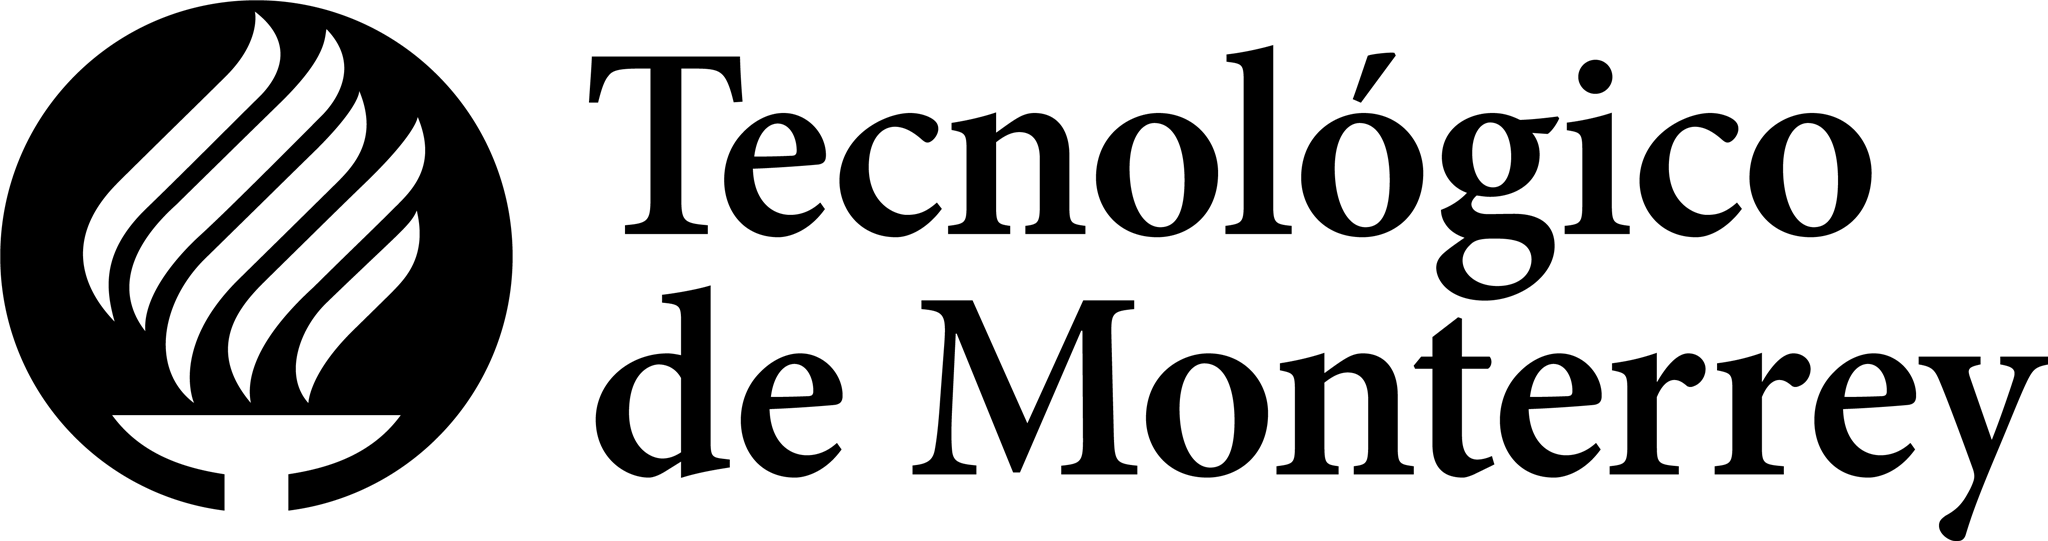
\includegraphics[width=0.4\textwidth,height=\textheight,keepaspectratio]{logo-tec-negro.png} % Include a department/university logo - this will require the graphicx package

    %----------------------------------------------------------------------------------------

    \vfill % Fill the rest of the page with whitespace

\end{titlepage}


\section{Problems}
Solve the following problems:
\begin{enumerate}
    \item For the selection algorithm, analyze and discuss the resulting complexity when the initial list is divided into groups of 19 elements (instead of 15). Derive the proper conclusions.\\
    The base equations are changed ass follows:
    \begin{align*}
        T(n) &= 58\frac{n}{19} + T'(n)\\
        T'(n) &= T(\frac{n}{19}) + 3(\frac{n}{19}) + 19(\frac{1}{2})(\frac{n}{38}) + T'(\frac{3}{4}n)\\
        T'(n) &= 58\frac{n}{19^2} + T'(\frac{n}{19}) + 3(\frac{n}{19}) + 19(\frac{1}{2})(\frac{n}{38}) + T'(\frac{3}{4}n)\\
        T'(n) &= 0.16066n +0.15789n + 0.25n + T'(\frac{n}{19}) + T'(\frac{3}{4}n)\\
        T'(n) &= 0.56855n + T'(\frac{n}{19}) + T'(\frac{3}{4}n)\\
        \alpha n &=0.56855n + \alpha \frac{n}{19} + \alpha \frac{3}{4}n\\
        \alpha &=0.56855 + \frac{\alpha}{19} + \alpha \frac{3}{4}\\
        \alpha &= 2.88\\
        T'(n) &\leq 2.88n\\
        T(n) &= 3.05n + 2.88n = 5.93n
    \end{align*}
    We can see that when the groups are contain 19 elements, the total complexity is reduced by a slight margin when compared to groups of 15 elements. We can also observe that in the 19 case, the way it's composed is different than in the 15 one. When you have 19 items in the group, the number of comparisons needed to find the quartile after broken and sorted is bigger, but the number of comparisons needed to find the $k^{th}$ quartile is smaller. This is clearly because the quartiles are bigger and for that, there are less groups to check.

    \item Given  a  set  of $n$ numbers,  we  want  to  find  the $i$ largest  in  sorted  order  using  a  comparison-based algorithm. Analyze and compare the following methods in terms of $n$ and $i$:
    \begin{enumerate}
        \item Sort the numbers, and list the $i$ largest.\\
        $O(nlog(n) + i )$
        \item Build a max-priority queue (like a heap) with the numbers and extract the minimum $i$ items.\\
        $O(nlog(n) + log(n) * i)$
        \item Use the k-max (session 06) to find the $i$-th largest, partition around that number, and sort the $i$ largest.
        $O(nlog(n) + (n-i)log(n - i))$
    \end{enumerate}

    \item For $n$ distinct elements $x_1, x_2, ..., x_n$ with positive weights $w_1, w_2, ..., w_n$ such that $\sum^{n}_{i=1} w_i= 1$, the weighted (lower) median is the element $x_k$ satisfying $\sum_{x_i<x_k}w_i < \frac{1}{2}$ and $\sum_{x_i>x_k}w_i \leq \frac{1}{2}$

    For example, if the elements are 0.1, 0.35, 0.05, 0.1, 0.15, 0.05, 0.2 and each element equals its weight then the median is 0.1, but the weighted median is 0.2.
    \begin{enumerate}
        \item Argue that the median of $x_1, x_2, ..., x_n$ is the weighted median of the $x_i$ with weights $w_i= 1/n$ for $i=1,2, ..., n$\\
        This is true, given that the median of a set of numbers is defined as the item in the middle when the set is sorted. This means that each one of the elements is as important as the next, ignoring its value or any other metric. This means that the weight of each one would be considered as $1/n$ and using the weighted sorted algorithm with this weight would yield the same result than the classical median.
        \item Show how to compute the weighted median of $n$ elements in $O(nlog(n))$ worst-case using sorting.\\
        For this, we would simply order the array, which gives us the term of $O(nlog(n))$ after which we would just add the weights until we find the one in which the sum surpasses 0.5, that would be the weighted median. That would take us at worst $O(n)$ time, and so the final result is that the complexity is $O(nlog(n))$.
        \item Show how to compute the weighted median of $n$ elements in $O(n)$ worst-case.\\
        First, you have to find the lower median, using the selection algorithm, it takes $O(n)$, then you partition the array in two parts split by the median which also costs $O(n)$. Then, you sum the weights of each part and check if the results meet the criteria layed above, again $O(n)$. If true, that's the weighted median, if not, you add the accumulated cost of the lighter part to the cost of the selected median and add it to the other part. Then apply the algorithm recursively in that partition. This all adds to a complexity of $O(n)$.
    \end{enumerate}

    \item Investigate on how the adversary argument concept can be used to determine the lower bound of merging two ordered lists.\\
    If we assume that there exists two sorted lists of size $n$, we can say that exists an algorithm $A$ that runs in $2n-2$ comparisons which merges the two lists correctly. Then, we say a list called $X$ contains the elements $x_i= 2i -1$ for $i=1$ to $n$ or odd numbers and a list $Y$ with elements $_i= 2i $ for $i=1$ to $n$ or even numbers. When we apply the algorithm $A$ in $X$ and $Y$. Because of the number of comparisons, we know that there exists an element of $X$, $x_i$ which was not compared to $y_i$ and $y_{i + 1}$. As such, there are two cases, that it was compared to $y_i$ or to $y_{i +1}$. In the first case, if we switch $x_i$ to $y_i$, the order of the lists will not be affected, but if we run the algorithm again, the resulting list will be wrong. Thus, there cannot exist any correct comparison-based algorithm that merges two sorted lists of size $n$ in less than $2n-1$ comparisons.
\end{enumerate}
\end{document}